%**************************************************************
% ARMA
%**************************************************************

\subsection{Auto Regressive Moving Average}
    In questa sezione esploriamo l'uso del modello univariato ARMA\cite{arma} 
    (Auto Regressive Moving Average) come 
    modello di riferimento che adotta un approccio statistico per valutare e confrontare l'efficacia del modello MSCRED\cite{mscred}.
    La scelta del modello ARMA è stata motivata principalmente dalla sua 
    utilizzazione da parte dei ricercatori di MSCRED per valutare le prestazioni di quest'ultimo. In generale, 
    ARMA è un modello ben consolidato e ampiamente utilizzato nella letteratura grazie alla sua semplice 
    implementazione e intuitività.

    Tuttavia, la sua semplicità ha un costo: il modello non è in grado di catturare l'intercorrelazione 
    tra i segnali perché è monovariato per natura. 
    Nell'esperimento presentato, per adattarsi alla natura monovariata del modello, è stato selezionato il
    segnale meno vuoto dal dataset di Infostud descritto nel \hyperref[cap2]{Capitolo 2}, ovvero il segnale con
    il minor numero, solo dieci, di valori nulli, avendo quindi a disposizione un totale di 48327 osservazioni.
    Il segnale interessato rappresenta la latenza media delle richieste di login a InfoSapienza.


    \paragraph{Intuizione} ARMA, nelle serie temporali, è utilizzato principalmente per la previsione di dati, ma 
    può essere usato anche per la rilevazione di anomalie. In linea generale, data una previsione di ARMA, i punti 
    in cui la previsione si discosta maggiormente rispetto ai punti originali vengono considerati anomalie.

    Più in dettaglio, ARMA effettua una certa previsione $P$ basata sui dati di training. Tale previsione viene 
    confrontata con i valori ground-truth $G$ calcolando i residui $P-G$. Attraverso l'iperparametro $t$ 
    vengono calcolati i confini decisionali $c^-, c^+$. ogni punto $i$ è valutato come anomalia se $P_i-G_i \notin [c^-, c^+]$,
    e non è valutato come tale altrimenti. 
    I confini decisionali $c^-, c^+$ sono ottenuti come segue: siano $\mu$ la media dei valori dell'unico segnale
    del dataset e sia $\sigma$ la sua deviazione standard: $c^+ = \mu + t^*\cdot\sigma, c^- = \mu - t^*\cdot\sigma$



    \paragraph{Dataset}Il dataset di Infostud è stato suddiviso in tre insiemi: training, validation e
    test, con percentuali rispettivamente pari a $0.5, 0.182, 0.318$. Allo scopo di 
    garantire una distribuzione accettabile delle anomalie nei tre insiemi, questa suddivisione atipica è stata 
    necessaria a causa della natura delle anomalie nel dataset, che sono principalmente di tipo collettivo 
    e quindi vicine tra loro sia nel tempo che nello spazio.
    Nel dataset, come già annunciato, è stato preso in considerazione un solo segnale, quello che rappresenta 
    la latenza media delle richieste di login effettuate a InfoSapienza, i cui dieci punti originariamente nulli 
    sono stati rimossi.
    Nella \hyperref[tab:dataset-arma]{Tabella 3.1.} sono riportate le informazioni in dettaglio della suddivisione 
    del dataset e nella \hyperref[fig:dataset-arma]{Figura 3.1.} è illustrato il dataset.

    \begin{table}[H]
        \centering
        \caption{Statistiche dataset ARMA (latenza media delle richieste di login).}
        \begin{tabular}{lccc}
            \toprule
            \textbf{Dataset} & \textbf{Indice di split} & \textbf{\# punti} & \textbf{Anomalie (\%)} \\
            \midrule
            \textbf{Training} & 0.5 & 24163 & 2.01 \% \\
            \textbf{Validation} & 0.182 & 8796 & 8.59 \% \\
            \textbf{Testing} & 0.318 & 15368 & 9.59 \% \\
            \bottomrule
        \end{tabular}
        \label{tab:dataset-arma}
    \end{table}

    \begin{figure}[H]
        \centering
        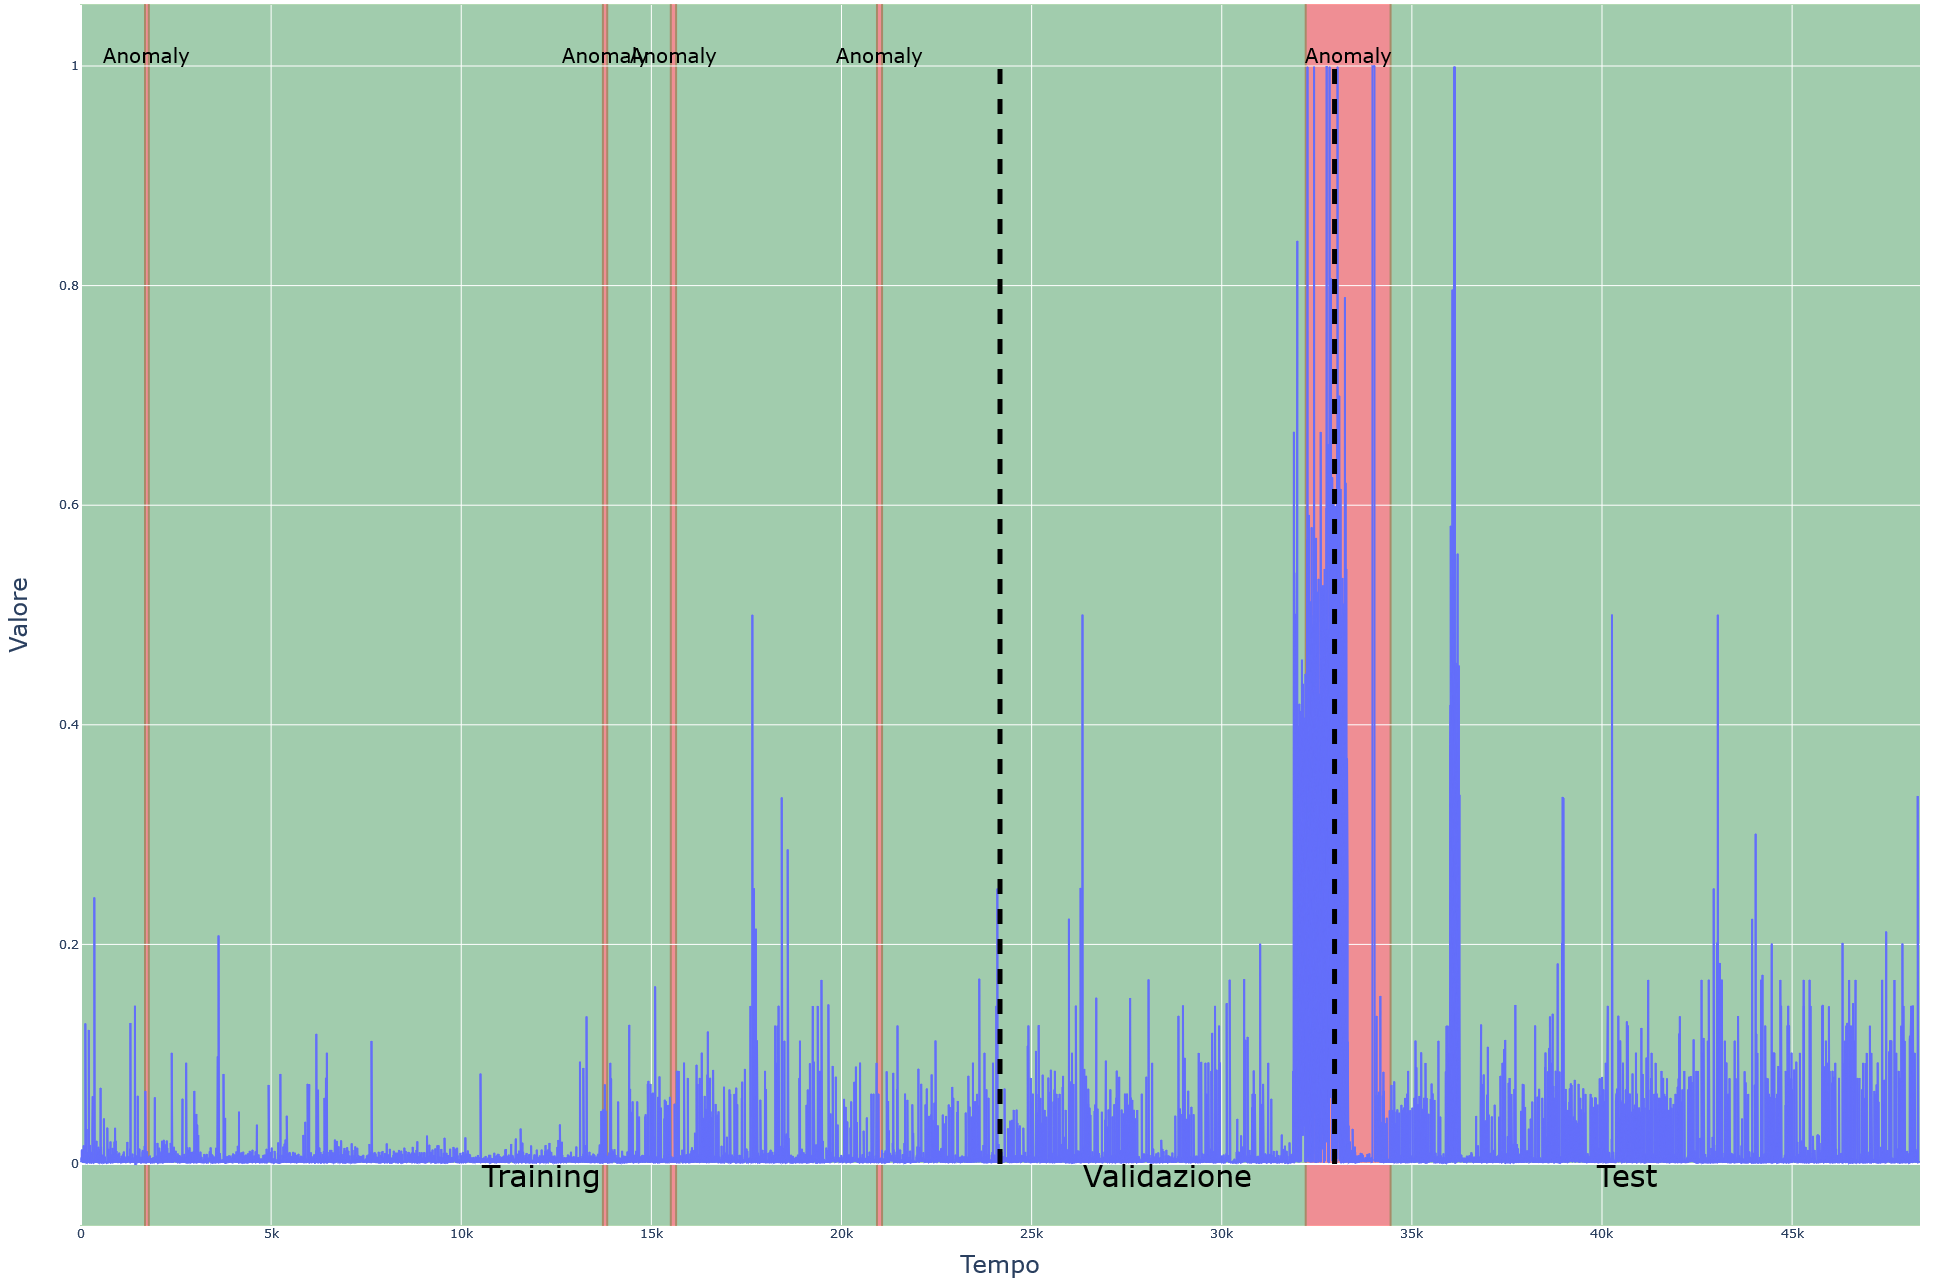
\includegraphics[width=0.6\textwidth]{./input/chapters/models/figs/arma-dataset.png}
        \caption{Dataset delle latenze medie alle richieste di login nel periodo 23 maggio - 22 giugno 2020. 
        Le bande rosse rappresentano le anomalie ground-truth, mentre quelle verdi i periodi non anomali. 
        Le linee tratteggiate delimitano il dataset di training da quello di validazione e quello di validazione dal test.}
        \label{fig:dataset-arma}
    \end{figure}

    \paragraph{Iperparametri} ARMA, in generale, presenta due iperparametri $p,q$. $p$ rappresenta l'ordine 
    dell'autoregressione nel modello ARMA. L'autoregressione si riferisce al fatto che il valore corrente 
    della serie temporale dipende dai valori passati della stessa serie temporale, in sintesi $p$ indica 
    quanti periodi temporali passati vengono utilizzati per predire il valore corrente ed è l'iperparametro 
    che fa sì che ARMA possa catturare le dipendenze temporali nella serie temporale. $q$, invece, 
    rappresenta l'ordine della media mobile nel modello. Essa indica che il valore della corrente serie 
    temporale dipende dai valori passati dei residui, ovvero degli errori previsionali, del modello stesso.
    Intuitivamente, $q$ indica quanti periodi temporali passati degli errori previsionali vengono utilizzati per 
    predire il valore corrente.

    Ai fini dell'anomaly detection, ARMA presenta anche un terzo iperparametro $t$ che, nel caso degli studi effettuati,
    è atto a creare i confini decisionali dei punti non anomali e, dualmente, anomali, definendo la sensibilità 
    del modello. 

    Per la scelta degli iperparametri è stata effettuata una grid-search di 30 epoche su $p$, $q$ e $t$  al fine di 
    individuare la combinazione che massimizzasse lo score F1, metrica illustrata nella \hyperref[f1-score]{Sottosezione 4.1.3}, 
    sul dataset di validation attraverso il training sul train set.

    Formalmente, siano $\mathbf{Tr}, \mathbf{Va}$ i dataset utilizzati per il training e
    per il validation rispettivamente, e sia $\text{ARMA}_\mathbf{X}^\mathbf{Y}$ un modello ARMA addestrato su 
    $\mathbf{X}$ che effettua previsioni nei punti $\mathbf{Y}$ e sia $T_{10}$ uno spazio lineare composto da 
    elementi equidistanti $t_i$ tali che $t_i \in [0.1, 5.0] \forall i \in [10]$:
    \begin{equation}
    \label{eq:arma-problem}
    \begin{aligned}
        & p^*, q^*, t^* = \max_{p, q, t} F1(\text{ARMA}_\mathbf{Tr}^\mathbf{Va}(p, q, t)) \\
        & \text{con il vincolo} \quad p, q \in [30], t \in T_{10}
    \end{aligned}
    \end{equation}


    \paragraph{Soluzione} \hyperref[eq:arma-problem]{L'equazione 3.1}  è stata soddisfatta dai seguenti:
    \begin{itemize}
        \item $p^* = 20$
        \item $q^* = 8$
        \item $t^* = 0.644$
    \end{itemize}

    Poiché l'insieme di validazione era necessario solo ai fini della ricerca degli iperparametri, è 
    stato successivamente accorpato al dataset di training. Dopo l'addestramento del modello sul nuovo dataset 
    con gli iperparametri che hanno generato una soluzione ottimale sul validation, sono state effettuate 
    le previsioni della serie temporale di test, mostrate nella \hyperref[fig:arma-sol]{Figura 3.2.}


    \begin{figure*}[h]
        \centering
        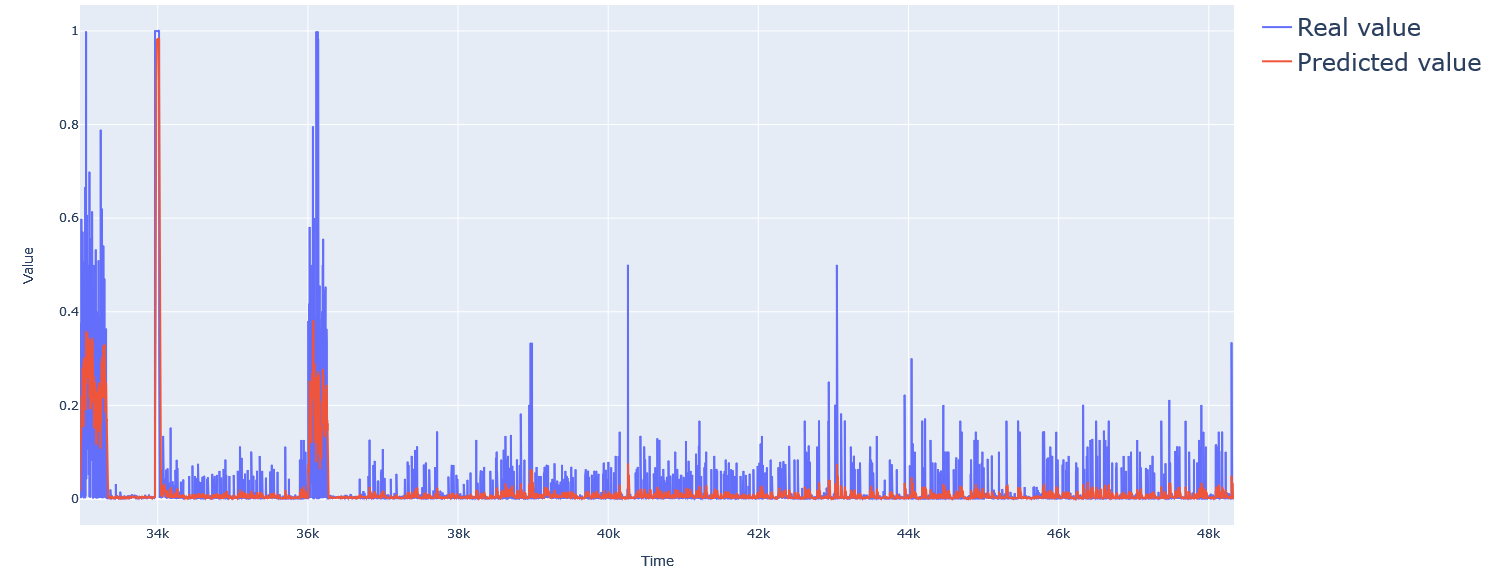
\includegraphics[width=0.7\textwidth]{./input/chapters/models/figs/arma-sol.png}
        \caption{Confronto della previsione del modello e le osservazioni originali sull'insieme di test.}
        \label{fig:arma-sol}
    \end{figure*}

    È evidente che il modello è in grado di prevedere l'andamento generale della serie temporale per la maggior
    parte del dataset. Tuttavia, in alcune aree, il modello presenta una performance inferiore rispetto ad altre.
    Queste aree saranno cruciali per la classificazione dei punti come anomali o non anomali.

    Sulla base delle previsioni $P$, sono stati calcolati i residui rispetto al test set $P-G$ e valutati come punti 
    anomali quelli che soddisfano $p_i-g_i \notin [c^-, c^+] | p_i \in P, g_i \in G$. I residui sono illustrati nella \hyperref[fig:residuals]{Figura 3.3.}

    I punti all'interno dell'intervallo definito dai confini inferiore e superiore non sono considerati anomali. 
    Tra questi punti ci sono quelli blu, che non sono anomalie e che il modello non ha considerato come tali
    (True Negatives), e quelli viola, che il modello ha erroneamente classificato come non anomalie (False Negatives).

    Possiamo inoltre osservare che svariati punti in verde sono sono stati correttamente classificati come anomalie
    (True Positives), ma sono presenti anche molti punti rossi, ovvero quelli che il modello ha erroneamente 
    considerato anomalie (False Positives). 

    \begin{figure}[H]
        \centering
        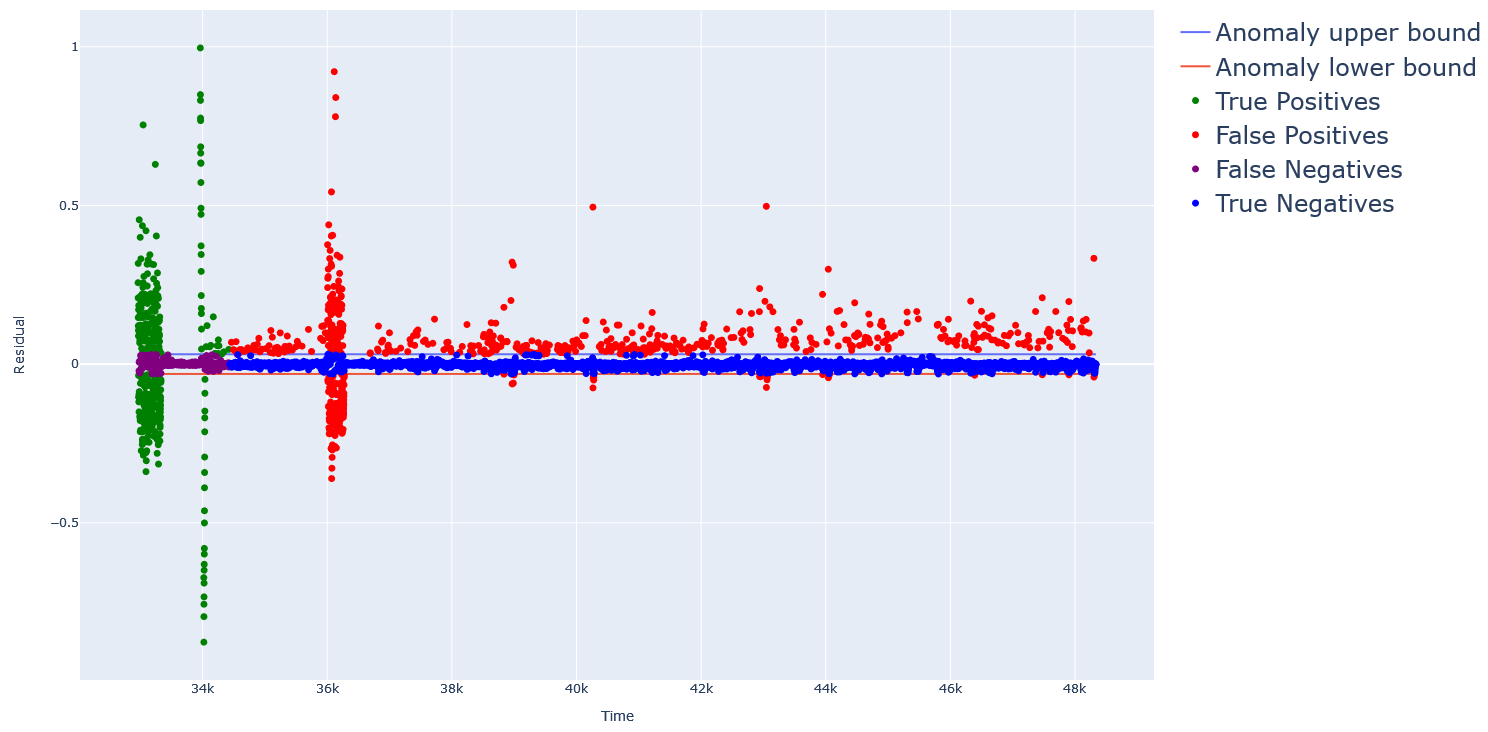
\includegraphics[width=0.7\textwidth]{./input/chapters/models/figs/arma-residuals.png}
        \caption{I residui del modello ARMA nel test set con i confini decisionali che discriminano la previsione delle 
        anomalie e le non anomalie.}
        \label{fig:residuals}
    \end{figure}